% Options for packages loaded elsewhere
\PassOptionsToPackage{unicode}{hyperref}
\PassOptionsToPackage{hyphens}{url}
\PassOptionsToPackage{dvipsnames,svgnames,x11names}{xcolor}
%
\documentclass[
  letterpaper,
  DIV=11,
  numbers=noendperiod]{scrartcl}

\usepackage{amsmath,amssymb}
\usepackage{iftex}
\ifPDFTeX
  \usepackage[T1]{fontenc}
  \usepackage[utf8]{inputenc}
  \usepackage{textcomp} % provide euro and other symbols
\else % if luatex or xetex
  \usepackage{unicode-math}
  \defaultfontfeatures{Scale=MatchLowercase}
  \defaultfontfeatures[\rmfamily]{Ligatures=TeX,Scale=1}
\fi
\usepackage{lmodern}
\ifPDFTeX\else  
    % xetex/luatex font selection
\fi
% Use upquote if available, for straight quotes in verbatim environments
\IfFileExists{upquote.sty}{\usepackage{upquote}}{}
\IfFileExists{microtype.sty}{% use microtype if available
  \usepackage[]{microtype}
  \UseMicrotypeSet[protrusion]{basicmath} % disable protrusion for tt fonts
}{}
\makeatletter
\@ifundefined{KOMAClassName}{% if non-KOMA class
  \IfFileExists{parskip.sty}{%
    \usepackage{parskip}
  }{% else
    \setlength{\parindent}{0pt}
    \setlength{\parskip}{6pt plus 2pt minus 1pt}}
}{% if KOMA class
  \KOMAoptions{parskip=half}}
\makeatother
\usepackage{xcolor}
\setlength{\emergencystretch}{3em} % prevent overfull lines
\setcounter{secnumdepth}{5}
% Make \paragraph and \subparagraph free-standing
\ifx\paragraph\undefined\else
  \let\oldparagraph\paragraph
  \renewcommand{\paragraph}[1]{\oldparagraph{#1}\mbox{}}
\fi
\ifx\subparagraph\undefined\else
  \let\oldsubparagraph\subparagraph
  \renewcommand{\subparagraph}[1]{\oldsubparagraph{#1}\mbox{}}
\fi

\usepackage{color}
\usepackage{fancyvrb}
\newcommand{\VerbBar}{|}
\newcommand{\VERB}{\Verb[commandchars=\\\{\}]}
\DefineVerbatimEnvironment{Highlighting}{Verbatim}{commandchars=\\\{\}}
% Add ',fontsize=\small' for more characters per line
\usepackage{framed}
\definecolor{shadecolor}{RGB}{241,243,245}
\newenvironment{Shaded}{\begin{snugshade}}{\end{snugshade}}
\newcommand{\AlertTok}[1]{\textcolor[rgb]{0.68,0.00,0.00}{#1}}
\newcommand{\AnnotationTok}[1]{\textcolor[rgb]{0.37,0.37,0.37}{#1}}
\newcommand{\AttributeTok}[1]{\textcolor[rgb]{0.40,0.45,0.13}{#1}}
\newcommand{\BaseNTok}[1]{\textcolor[rgb]{0.68,0.00,0.00}{#1}}
\newcommand{\BuiltInTok}[1]{\textcolor[rgb]{0.00,0.23,0.31}{#1}}
\newcommand{\CharTok}[1]{\textcolor[rgb]{0.13,0.47,0.30}{#1}}
\newcommand{\CommentTok}[1]{\textcolor[rgb]{0.37,0.37,0.37}{#1}}
\newcommand{\CommentVarTok}[1]{\textcolor[rgb]{0.37,0.37,0.37}{\textit{#1}}}
\newcommand{\ConstantTok}[1]{\textcolor[rgb]{0.56,0.35,0.01}{#1}}
\newcommand{\ControlFlowTok}[1]{\textcolor[rgb]{0.00,0.23,0.31}{#1}}
\newcommand{\DataTypeTok}[1]{\textcolor[rgb]{0.68,0.00,0.00}{#1}}
\newcommand{\DecValTok}[1]{\textcolor[rgb]{0.68,0.00,0.00}{#1}}
\newcommand{\DocumentationTok}[1]{\textcolor[rgb]{0.37,0.37,0.37}{\textit{#1}}}
\newcommand{\ErrorTok}[1]{\textcolor[rgb]{0.68,0.00,0.00}{#1}}
\newcommand{\ExtensionTok}[1]{\textcolor[rgb]{0.00,0.23,0.31}{#1}}
\newcommand{\FloatTok}[1]{\textcolor[rgb]{0.68,0.00,0.00}{#1}}
\newcommand{\FunctionTok}[1]{\textcolor[rgb]{0.28,0.35,0.67}{#1}}
\newcommand{\ImportTok}[1]{\textcolor[rgb]{0.00,0.46,0.62}{#1}}
\newcommand{\InformationTok}[1]{\textcolor[rgb]{0.37,0.37,0.37}{#1}}
\newcommand{\KeywordTok}[1]{\textcolor[rgb]{0.00,0.23,0.31}{#1}}
\newcommand{\NormalTok}[1]{\textcolor[rgb]{0.00,0.23,0.31}{#1}}
\newcommand{\OperatorTok}[1]{\textcolor[rgb]{0.37,0.37,0.37}{#1}}
\newcommand{\OtherTok}[1]{\textcolor[rgb]{0.00,0.23,0.31}{#1}}
\newcommand{\PreprocessorTok}[1]{\textcolor[rgb]{0.68,0.00,0.00}{#1}}
\newcommand{\RegionMarkerTok}[1]{\textcolor[rgb]{0.00,0.23,0.31}{#1}}
\newcommand{\SpecialCharTok}[1]{\textcolor[rgb]{0.37,0.37,0.37}{#1}}
\newcommand{\SpecialStringTok}[1]{\textcolor[rgb]{0.13,0.47,0.30}{#1}}
\newcommand{\StringTok}[1]{\textcolor[rgb]{0.13,0.47,0.30}{#1}}
\newcommand{\VariableTok}[1]{\textcolor[rgb]{0.07,0.07,0.07}{#1}}
\newcommand{\VerbatimStringTok}[1]{\textcolor[rgb]{0.13,0.47,0.30}{#1}}
\newcommand{\WarningTok}[1]{\textcolor[rgb]{0.37,0.37,0.37}{\textit{#1}}}

\providecommand{\tightlist}{%
  \setlength{\itemsep}{0pt}\setlength{\parskip}{0pt}}\usepackage{longtable,booktabs,array}
\usepackage{calc} % for calculating minipage widths
% Correct order of tables after \paragraph or \subparagraph
\usepackage{etoolbox}
\makeatletter
\patchcmd\longtable{\par}{\if@noskipsec\mbox{}\fi\par}{}{}
\makeatother
% Allow footnotes in longtable head/foot
\IfFileExists{footnotehyper.sty}{\usepackage{footnotehyper}}{\usepackage{footnote}}
\makesavenoteenv{longtable}
\usepackage{graphicx}
\makeatletter
\def\maxwidth{\ifdim\Gin@nat@width>\linewidth\linewidth\else\Gin@nat@width\fi}
\def\maxheight{\ifdim\Gin@nat@height>\textheight\textheight\else\Gin@nat@height\fi}
\makeatother
% Scale images if necessary, so that they will not overflow the page
% margins by default, and it is still possible to overwrite the defaults
% using explicit options in \includegraphics[width, height, ...]{}
\setkeys{Gin}{width=\maxwidth,height=\maxheight,keepaspectratio}
% Set default figure placement to htbp
\makeatletter
\def\fps@figure{htbp}
\makeatother

\KOMAoption{captions}{tableheading}
\makeatletter
\makeatother
\makeatletter
\makeatother
\makeatletter
\@ifpackageloaded{caption}{}{\usepackage{caption}}
\AtBeginDocument{%
\ifdefined\contentsname
  \renewcommand*\contentsname{Tabla de contenidos}
\else
  \newcommand\contentsname{Tabla de contenidos}
\fi
\ifdefined\listfigurename
  \renewcommand*\listfigurename{Listado de Figuras}
\else
  \newcommand\listfigurename{Listado de Figuras}
\fi
\ifdefined\listtablename
  \renewcommand*\listtablename{Listado de Tablas}
\else
  \newcommand\listtablename{Listado de Tablas}
\fi
\ifdefined\figurename
  \renewcommand*\figurename{Figura}
\else
  \newcommand\figurename{Figura}
\fi
\ifdefined\tablename
  \renewcommand*\tablename{Tabla}
\else
  \newcommand\tablename{Tabla}
\fi
}
\@ifpackageloaded{float}{}{\usepackage{float}}
\floatstyle{ruled}
\@ifundefined{c@chapter}{\newfloat{codelisting}{h}{lop}}{\newfloat{codelisting}{h}{lop}[chapter]}
\floatname{codelisting}{Listado}
\newcommand*\listoflistings{\listof{codelisting}{Listado de Listados}}
\makeatother
\makeatletter
\@ifpackageloaded{caption}{}{\usepackage{caption}}
\@ifpackageloaded{subcaption}{}{\usepackage{subcaption}}
\makeatother
\makeatletter
\@ifpackageloaded{tcolorbox}{}{\usepackage[skins,breakable]{tcolorbox}}
\makeatother
\makeatletter
\@ifundefined{shadecolor}{\definecolor{shadecolor}{rgb}{.97, .97, .97}}
\makeatother
\makeatletter
\makeatother
\makeatletter
\makeatother
\ifLuaTeX
\usepackage[bidi=basic]{babel}
\else
\usepackage[bidi=default]{babel}
\fi
\babelprovide[main,import]{spanish}
% get rid of language-specific shorthands (see #6817):
\let\LanguageShortHands\languageshorthands
\def\languageshorthands#1{}
\ifLuaTeX
  \usepackage{selnolig}  % disable illegal ligatures
\fi
\IfFileExists{bookmark.sty}{\usepackage{bookmark}}{\usepackage{hyperref}}
\IfFileExists{xurl.sty}{\usepackage{xurl}}{} % add URL line breaks if available
\urlstyle{same} % disable monospaced font for URLs
\hypersetup{
  pdftitle={Curso de Django},
  pdfauthor={Lcdo. Diego Medardo Saavedra García. Mgtr.},
  pdflang={es},
  colorlinks=true,
  linkcolor={blue},
  filecolor={Maroon},
  citecolor={Blue},
  urlcolor={Blue},
  pdfcreator={LaTeX via pandoc}}

\title{Curso de Django}
\usepackage{etoolbox}
\makeatletter
\providecommand{\subtitle}[1]{% add subtitle to \maketitle
  \apptocmd{\@title}{\par {\large #1 \par}}{}{}
}
\makeatother
\subtitle{Módulo 1: Introducción a Django}
\author{Lcdo. Diego Medardo Saavedra García. Mgtr.}
\date{2023-07-19}

\begin{document}
\maketitle
\ifdefined\Shaded\renewenvironment{Shaded}{\begin{tcolorbox}[boxrule=0pt, enhanced, frame hidden, borderline west={3pt}{0pt}{shadecolor}, sharp corners, interior hidden, breakable]}{\end{tcolorbox}}\fi

\renewcommand*\contentsname{Tabla de contenidos}
{
\hypersetup{linkcolor=}
\setcounter{tocdepth}{3}
\tableofcontents
}
\hypertarget{muxf3dulo-1-introducciuxf3n-a-django.}{%
\section{Módulo 1: Introducción a
Django.}\label{muxf3dulo-1-introducciuxf3n-a-django.}}

\hypertarget{quuxe9-es-django-y-por-quuxe9-utilizarlo}{%
\subsection{¿Qué es Django y por qué
utilizarlo?}\label{quuxe9-es-django-y-por-quuxe9-utilizarlo}}

\begin{itemize}
\tightlist
\item
  Django es un framework web de alto nivel basado en Python.
\item
  Facilita el desarrollo rápido de aplicaciones web robustas y seguras.
\item
  Ventajas de Django: MVC (Modelo-Vista-Controlador), administrador de
  base de datos, seguridad integrada y comunidad activa.
\end{itemize}

\hypertarget{mvc-xvs-mtv.}{%
\subsection{MVC x`vs MTV.}\label{mvc-xvs-mtv.}}

\begin{longtable}[]{@{}
  >{\centering\arraybackslash}p{(\columnwidth - 0\tabcolsep) * \real{0.7361}}@{}}
\toprule\noalign{}
\endhead
\bottomrule\noalign{}
\endlastfoot
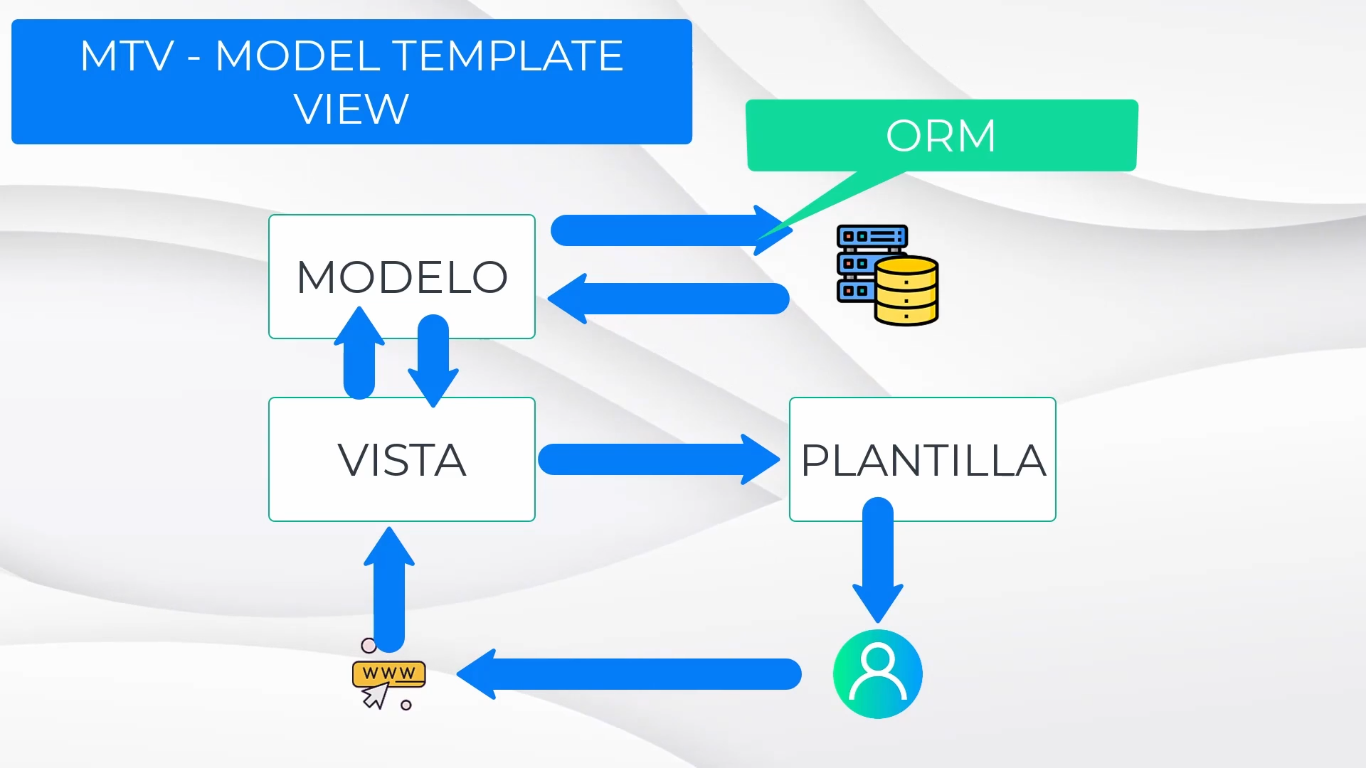
\includegraphics{images/img001.png} \\
\end{longtable}

\hypertarget{instalaciuxf3n-de-django-4.2.3-y-configuraciuxf3n-del-entorno-de-desarrollo}{%
\subsection{Instalación de Django 4.2.3 y Configuración del Entorno de
Desarrollo}\label{instalaciuxf3n-de-django-4.2.3-y-configuraciuxf3n-del-entorno-de-desarrollo}}

Para instalar Django 4.2.3, se recomienda utilizar un entorno virtual
(por ejemplo, con virtualenv o conda).

Comandos para instalar Django y crear un entorno virtual:

\begin{Shaded}
\begin{Highlighting}[]
\CommentTok{\# Instalación de virtualenv}

\ExtensionTok{pip}\NormalTok{ install virtualenv}

\CommentTok{\# Creación del entorno virtual}

\ExtensionTok{python} \AttributeTok{{-}m}\NormalTok{ venv env}

\CommentTok{\# Activación del Entorno Virtual}

\BuiltInTok{cd}\NormalTok{ env/Scripts}
\ExtensionTok{activate}

\CommentTok{\# Salir del directorio Scripts}
\BuiltInTok{cd}\NormalTok{ ../../}

\CommentTok{\# Instalación de Django usando pip}
\ExtensionTok{pip}\NormalTok{ install django==4.2.3}
\end{Highlighting}
\end{Shaded}

\hypertarget{creaciuxf3n-de-un-proyecto-en-django.}{%
\subsection{Creación de un Proyecto en
Django.}\label{creaciuxf3n-de-un-proyecto-en-django.}}

Para crear un nuevo proyecto Django, utilizamos el comando

\begin{Shaded}
\begin{Highlighting}[]
\ExtensionTok{django{-}admin}\NormalTok{ startproject nombre\_proyecto .}
\end{Highlighting}
\end{Shaded}

\hypertarget{estructura-de-directorios-generada}{%
\subsubsection{Estructura de directorios
generada:}\label{estructura-de-directorios-generada}}

\begin{Shaded}
\begin{Highlighting}[]
\NormalTok{nombre\_proyecto/}
\NormalTok{    manage.py}
\NormalTok{        \_\_init\_\_.py}
\NormalTok{        settings.py}
\NormalTok{        urls.py}
\NormalTok{        asgi.py}
\NormalTok{        wsgi.py}
\end{Highlighting}
\end{Shaded}

\hypertarget{estructura-de-directorios-de-un-proyecto-django.}{%
\subsubsection{Estructura de Directorios de un Proyecto
Django.}\label{estructura-de-directorios-de-un-proyecto-django.}}

La estructura de directorios de un proyecto Django se organiza de la
siguiente manera:

\begin{Shaded}
\begin{Highlighting}[]

\NormalTok{nombre\_proyecto/}
\NormalTok{│   manage.py}
\NormalTok{│}
\NormalTok{└───nombre\_proyecto/}
\NormalTok{│   │   \_\_init\_\_.py}
\NormalTok{│   │   settings.py}
\NormalTok{│   │   urls.py}
\NormalTok{│   │   asgi.py}
\NormalTok{│   │   wsgi.py}
\NormalTok{│}
\NormalTok{└───otras\_aplicaciones/}
\NormalTok{    │   ...}
\end{Highlighting}
\end{Shaded}

\begin{longtable}[]{@{}
  >{\centering\arraybackslash}p{(\columnwidth - 2\tabcolsep) * \real{0.2361}}
  >{\centering\arraybackslash}p{(\columnwidth - 2\tabcolsep) * \real{0.7361}}@{}}
\toprule\noalign{}
\begin{minipage}[b]{\linewidth}\centering
Directorio y/o Archivo
\end{minipage} & \begin{minipage}[b]{\linewidth}\centering
Descripción
\end{minipage} \\
\midrule\noalign{}
\endhead
\bottomrule\noalign{}
\endlastfoot
\textbf{nomb re\_proyecto/} & Es el directorio raíz del proyecto.
Contiene el archivo ``manage.py'', que es una herramienta para
administrar el proyecto y ejecutar comandos de Django. \\
\begin{minipage}[t]{\linewidth}\centering
\begin{itemize}
\tightlist
\item
  *nombre\_proyec to/nomb re\_proyecto/**
\end{itemize}
\end{minipage} & Es el directorio de la configuración del proyecto.
Contiene varios archivos esenciales: \\
\textbf{init.py} & Este archivo indica a Python que el directorio es un
paquete y permite la importación de módulos dentro de él. \\
\begin{minipage}[t]{\linewidth}\centering
\begin{itemize}
\tightlist
\item
  *settings.py**
\end{itemize}
\end{minipage} & Aquí se encuentran todas las configuraciones del
proyecto, como bases de datos, aplicaciones instaladas, rutas de
plantillas, configuraciones de seguridad, etc. \\
\textbf{urls.py} & Contiene las configuraciones de las URLs del
proyecto, es decir, cómo se manejan las solicitudes y se mapean a las
vistas. \\
\textbf{asgi.py} y \textbf{wsgi.py} & Son archivos de configuración para
el servidor ASGI (Asynchronous Server Gateway Interface) y WSGI (Web
Server Gateway Interface), respectivamente. Estos archivos son
utilizados por servidores web para servir la aplicación Django. \\
\textbf{otras\_a plicaciones/} & Es un directorio opcional donde puedes
organizar las aplicaciones adicionales que desarrolles para el proyecto.
Cada aplicación puede tener su propia estructura de directorios. \\
\end{longtable}

\hypertarget{creaciuxf3n-de-una-aplicaciuxf3n-en-django}{%
\subsection{Creación de una Aplicación en
Django}\label{creaciuxf3n-de-una-aplicaciuxf3n-en-django}}

Una aplicación es un componente reutilizable de un proyecto Django.
Comando para crear una nueva aplicación:

\begin{Shaded}
\begin{Highlighting}[]
\ExtensionTok{python}\NormalTok{ manage.py startapp nombre\_app}
\end{Highlighting}
\end{Shaded}

Estructura de directorios de una aplicación:

\begin{Shaded}
\begin{Highlighting}[]
\NormalTok{nombre\_app/}
\NormalTok{│   migrations/}
\NormalTok{│   │   ...}
\NormalTok{│   │   \_\_init\_\_.py}
\NormalTok{│   │}
\NormalTok{│   │   admin.py}
\NormalTok{│   │   apps.py}
\NormalTok{│   │   models.py}
\NormalTok{│   │   tests.py}
\NormalTok{│   │   views.py}
\end{Highlighting}
\end{Shaded}

\begin{longtable}[]{@{}
  >{\raggedright\arraybackslash}p{(\columnwidth - 2\tabcolsep) * \real{0.2361}}
  >{\centering\arraybackslash}p{(\columnwidth - 2\tabcolsep) * \real{0.7361}}@{}}
\toprule\noalign{}
\begin{minipage}[b]{\linewidth}\raggedright
Directorio y/o Archivo
\end{minipage} & \begin{minipage}[b]{\linewidth}\centering
Descripción
\end{minipage} \\
\midrule\noalign{}
\endhead
\bottomrule\noalign{}
\endlastfoot
nombre\_app & Es el directorio raíz de la aplicación. Contiene los
archivos esenciales y directorios para el funcionamiento de la
aplicación. \\
migrations/ & Es un directorio generado automáticamente por Django
cuando se realizan cambios en los modelos de la aplicación. Contiene
archivos de migración que representan los cambios en la base de
datos. \\
init.py & Este archivo indica a Python que el directorio es un paquete y
permite la importación de módulos dentro de él. \\
admin.py & En este archivo se pueden registrar los modelos de la
aplicación para que aparezcan en el panel de administración de
Django. \\
apps.py & Es el archivo donde se define la configuración de la
aplicación, como su nombre y configuraciones adicionales. \\
models.py & Aquí se definen los modelos de la aplicación utilizando la
clase ``Model'' de Django. Los modelos representan las tablas en la base
de datos y definen los campos y relaciones de la aplicación. \\
tests.py & Es el archivo donde se pueden escribir pruebas unitarias y de
integración para la aplicación. \\
views.py & Contiene las vistas de la aplicación, que son funciones o
clases que manejan las solicitudes y generan las respuestas. Las vistas
determinan qué se muestra en las páginas web de la aplicación. \\
\end{longtable}

\hypertarget{ejemplo-pruxe1ctico}{%
\section{Ejemplo Práctico:}\label{ejemplo-pruxe1ctico}}

\hypertarget{creaciuxf3n-de-un-proyecto-de-e-commerce-en-django}{%
\subsection{Creación de un Proyecto de E-commerce en
Django}\label{creaciuxf3n-de-un-proyecto-de-e-commerce-en-django}}

En esta actividad práctica, crearás un nuevo proyecto de e-commerce en
Django desde cero. Asegúrate de tener Django instalado en tu entorno de
desarrollo antes de comenzar.

\textbf{Paso 1:} Crear un Proyecto de Django

Abre una terminal o línea de comandos en la ubicación donde desees crear
tu proyecto de e-commerce.

Ejecuta el siguiente comando para crear un nuevo proyecto Django llamado
``mi\_ecommerce'':

\begin{Shaded}
\begin{Highlighting}[]
\ExtensionTok{django{-}admin}\NormalTok{ startproject mi\_ecommerce}
\end{Highlighting}
\end{Shaded}

Verás que se ha creado un nuevo directorio llamado ``mi\_ecommerce'' que
contiene la estructura inicial del proyecto.

\textbf{Paso 2:} Crear una Aplicación para el E-commerce

Cambia al directorio recién creado ``mi\_ecommerce'':

\begin{Shaded}
\begin{Highlighting}[]
\BuiltInTok{cd}\NormalTok{ mi\_ecommerce}
\end{Highlighting}
\end{Shaded}

Ahora, crea una nueva aplicación llamada ``ecommerce'' utilizando el
siguiente comando:

\begin{Shaded}
\begin{Highlighting}[]
\ExtensionTok{python}\NormalTok{ manage.py startapp ecommerce}
\end{Highlighting}
\end{Shaded}

Se creará un nuevo directorio ``ecommerce'' dentro de tu proyecto, que
contendrá todos los archivos necesarios para la aplicación.

\textbf{Paso 3:} Configurar el Proyecto y la Aplicación

Abre el archivo ``settings.py'' ubicado en el directorio
``mi\_ecommerce/mi\_ecommerce''.

Asegúrate de agregar la aplicación ``ecommerce'' en la lista de
``INSTALLED\_APPS'' para que Django la reconozca:

\begin{Shaded}
\begin{Highlighting}[]
\NormalTok{INSTALLED\_APPS }\OperatorTok{=}\NormalTok{ [}
    \CommentTok{\# Otras aplicaciones...}
    \StringTok{\textquotesingle{}ecommerce\textquotesingle{}}\NormalTok{,}
\NormalTok{]}
\end{Highlighting}
\end{Shaded}

\textbf{Paso 4:} Ejecutar el Servidor de Desarrollo

Ahora, ejecuta el servidor de desarrollo para ver el proyecto en acción:

\begin{Shaded}
\begin{Highlighting}[]
\ExtensionTok{python}\NormalTok{ manage.py runserver}
\end{Highlighting}
\end{Shaded}

Abre tu navegador y visita la dirección
``\url{http://localhost:8000/}''. Deberías ver la página de bienvenida
de Django.

Si has llegado a este punto, ¡Felicidades! Has creado con éxito un nuevo
proyecto de e-commerce en Django y una aplicación llamada ``ecommerce''.
Ahora puedes comenzar a desarrollar las funcionalidades del e-commerce y
diseñar las diapositivas para cada uno de los módulos del curso.

¡Buena suerte!

\hypertarget{actividad-pruxe1ctica.}{%
\section{Actividad Práctica.}\label{actividad-pruxe1ctica.}}

\hypertarget{creaciuxf3n-de-un-blog}{%
\subsection{Creación de Un Blog}\label{creaciuxf3n-de-un-blog}}

En esta actividad práctica, crearás un nuevo proyecto de Blog en Django
desde cero. Asegúrate de tener Django instalado en tu entorno de
desarrollo antes de comenzar.

\textbf{Paso 1:} Crear un Proyecto de Django

\textbf{Paso 2:} Crear una Aplicación para el E-commerce

\textbf{Paso 3:} Configurar el Proyecto y la Aplicación

\textbf{Paso 4:} Ejecutar el Servidor de Desarrollo

\hypertarget{resoluciuxf3n-de-la-actividad-pruxe1ctica}{%
\subsection{Resolución de la Actividad
Práctica:}\label{resoluciuxf3n-de-la-actividad-pruxe1ctica}}

En esta actividad práctica, crearás un nuevo proyecto de blog en Django
desde cero. Asegúrate de tener Django instalado en tu entorno de
desarrollo antes de comenzar.

\textbf{Paso 1:} Crear un Proyecto de Django

Abre una terminal o línea de comandos en la ubicación donde desees crear
tu proyecto de blog.

Ejecuta el siguiente comando para crear un nuevo proyecto Django llamado
``mi\_blog'':

\begin{Shaded}
\begin{Highlighting}[]
\ExtensionTok{django{-}admin}\NormalTok{ startproject mi\_blog}
\end{Highlighting}
\end{Shaded}

Verás que se ha creado un nuevo directorio llamado ``mi\_blog'' que
contiene la estructura inicial del proyecto.

\textbf{Paso 2:} Crear una Aplicación para el Blog

Cambia al directorio recién creado ``mi\_blog'':

\begin{Shaded}
\begin{Highlighting}[]
\BuiltInTok{cd}\NormalTok{ mi\_blog}
\end{Highlighting}
\end{Shaded}

Ahora, crea una nueva aplicación llamada ``blog'' utilizando el
siguiente comando:

\begin{Shaded}
\begin{Highlighting}[]
\ExtensionTok{python}\NormalTok{ manage.py startapp blog}
\end{Highlighting}
\end{Shaded}

Se creará un nuevo directorio ``blog'' dentro de tu proyecto, que
contendrá todos los archivos necesarios para la aplicación.

\textbf{Paso 3:} Configurar el Proyecto y la Aplicación

Abre el archivo ``settings.py'' ubicado en el directorio
``mi\_blog/mi\_blog''.

Asegúrate de agregar la aplicación ``blog'' en la lista de
``INSTALLED\_APPS'' para que Django la reconozca:

\begin{Shaded}
\begin{Highlighting}[]
\NormalTok{INSTALLED\_APPS }\OperatorTok{=}\NormalTok{ [}
    \CommentTok{\# Otras aplicaciones...}
    \StringTok{\textquotesingle{}blog\textquotesingle{}}\NormalTok{,}
\NormalTok{]}
\end{Highlighting}
\end{Shaded}

\textbf{Paso 4:} Ejecutar el Servidor de Desarrollo

Ahora, ejecuta el servidor de desarrollo para ver el proyecto en acción:

\begin{Shaded}
\begin{Highlighting}[]
\ExtensionTok{python}\NormalTok{ manage.py runserver}
\end{Highlighting}
\end{Shaded}

Abre tu navegador y visita la dirección ``http://localhost:8000/''.
Deberías ver la página de bienvenida de Django.

¡Felicidades! Has creado con éxito un nuevo proyecto de blog en Django y
una aplicación llamada ``blog''. Ahora puedes comenzar a desarrollar las
funcionalidades del blog y diseñar las diapositivas para cada uno de los
módulos del curso. ¡Buena suerte!



\end{document}
